\todo{Zaktualizować opis algorytmu od strony teoretycznej}
Korzystając z~wiedzy i~doświadczeń wyniesionych z~sekcji~\ref{sec:przeglad} niniejszego sprawozdania, zdecydowaliśmy się na stworzenie systemu odpowiadającego na pytania ogólne, z~wyszczególnieniem pytań o~fakty dotyczące:
\begin{itemize}
    \item osób,
    \item miejsc,
    \item dat,
    \item cech wielkościowych,
    \item przedmiotów.
\end{itemize}

Bazą więdzy systemu będzie sieć WWW. Do wyszukiwania dokumentów w~sieci~WWW, wykorzystane zostaną wyszukiwarki internetowe: \emph{Google\footnote{www.google.pl}}, \emph{Bing\footnote{www.bing.com}}, \emph{Yahoo\footnote{www.search.yahoo.com}} oraz \emph{DuckDuckGo\footnote{duckduckgo.com}}. Podobnie jak we wcześniej omawianym systemie AskMSR~\cite{brill2002analysis}, do dalszej analizy przekazywane będą jedynie \emph{snippety}, co pozwoli na uproszczenie etapu filtracji akapitów.

Odpowiedzią na przedstawione pytanie, będzie prosta odpowiedź typu \emph{Named-Entity}. Nie przewidujemy odpowiadania na pytania w~języku naturalnym.

\subsection{Zarys algorytmu}
Na rysunku~\ref{fig:algorithm-overview}, przedstawiony został ogólny schemat algorytmu odpowiadania na pytania.

\begin{figure}[h]
    \centering
    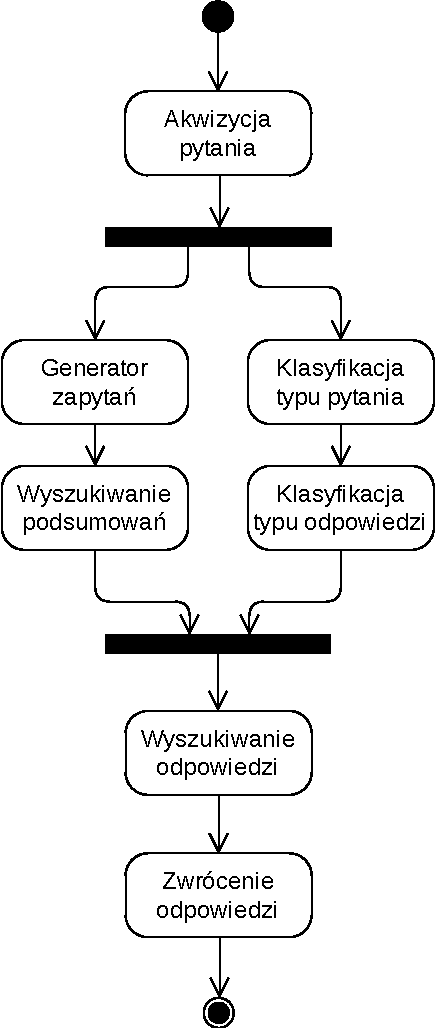
\includegraphics[width=0.7\columnwidth]{figures/WEDT-Algorytm.pdf}
    \caption{Ogólny schemat algorytmu odpowiadania na pytania}
    \label{fig:algorithm-overview}
\end{figure}

Pierwszym krokiem algorytmu jest akwizycja pytania od użytkownika systemu. Każde pytanie będzie analizowane w~sposób indywidualny, bez przechowywania wcześniejszych pytań i~utrzymywania kontekstu. Nie zakładamy również żadnego profilowania użytkowników, ponieważ typowo proste pytania o~fakty, są ze sobą słabo powiązane.

W~kolejnym kroku, strumień sterowania rozdwaja się i~jest przekazywany do dwóch modułów, które przetwarzają zapytanie równolegle. Moduł akwizycji wiedzy, na podstawie przekazanego pytania, stara się uzyskać jak największą ilość \emph{snippetów}, generując specjalistyczne zapytania do każdej z~czterech wyszukiwarek, tak jak to zostało przedstawione w~\cite{zheng2002answerbus}. Oprócz tego, aby wykorzystać redundantość sieci~WWW, do wyszukiwarek wysłane zostaną również okrojone zapytania, pozbawione części słów, tak aby zwiększyć zakres poszukiwań, podobnie jak w~\cite{brill2002analysis}. Aby zwiększyć rozmiar zbioru wyszukanych \emph{snippetów}, słowa kluczowe w~zapytaniu, będą wymieniane na ich synonimy~\cite{przybyla-2013-question}.

W~trakcie wyszukiwania \emph{snippetów}, w~drugiej gałęzi algorytmu, następuję klasyfikacja typu pytania i~oczekiwanej odpowiedzi. Klasy pytań są definiowane przez zaimki pytające, podobnie jak w~\cite{gupta2012survey}. Wyróżniamy pytania typu: \emph{Kto?}, \emph{Jaki/Jaka/Jakie?}, \emph{Jak?}, \emph{Gdzie?}, \emph{Kiedy?}, \emph{Co?} oraz \emph{Który/Która/Które?}. Wykrywanie typu pytania odbywać się będzie w~prosty sposób, stosując reguły podstawieniowe oraz rozkład zdania. Określanie typu oczekiwanej odpowiedzi będzie wynikało głównie z~typu pytania, wspartej możliwością odpytania usługi \emph{plWordNet}~\cite{MazPiaRudSzpaKedz:16} oraz dodatkowym sprawdzeniem wyrażeń regularnych.

Każdy wyszukany \emph{snippet} zostanie poddany analizie morfologicznej, po której przyporządkowana zostanie mu odpowiednia ocena. W~każdym zdaniu, za pomocą taggera oraz \emph{plWordNetu} wyszukiwane będą \emph{Named-Entities}, które mogą stanowić potencjalną odpowiedź na pytanie. Ostatnim krokiem procesu będzie zwrócenie najlepszej odpowiedzi lub zbioru najlepszych odpowiedzi. Do odpowiedzi dołączony może zostać link ze źródłem, w~celu umożliwienia użytkownikowi systemu osobistej weryfikacji odpowiedzi.

